\documentclass[conference]{IEEEtran}
\usepackage[T1]{fontenc}
\usepackage{amsmath,amssymb}
\usepackage{graphicx}
\usepackage{booktabs}
\usepackage{url}
\usepackage[hidelinks]{hyperref}
\graphicspath{{../figures/}}

\begin{document}

\title{Recall Under Paraphrase for Trust-Locked Patient Memory: A Blind Benchmark, Hybrid Lexical--Embedding Matching and Training-Free Hand-Set Heads}

\author{\IEEEauthorblockN{Faaz Khan Mohammad}
\IEEEauthorblockA{Rapport project\\
Email: faazkhn1000@gmail.com}}

\maketitle

\begin{abstract}
A simulated psychiatric patient must recognise which of its memories a trainee's question touches before deciding whether trust
allows it to answer. Keyword tags miss paraphrases, and in a patient simulator each missed risk question is a safety defect: a
version that failed to match ``thoughts that life isn't worth living'' denied a death wish it should have disclosed. We built a blind
benchmark of 512 doctor lines over four psychiatric cases, written from each fact's clinical meaning by a writer who never saw the
tags, split into a tuning half and a test half. Keyword recall found 35.1\% of risk-fact questions on the test half. Hybrid matching
(keyword tags plus a 33-million-parameter sentence encoder over authored and generated probe questions, with trust locks applied
after matching) found 72.7\% at 15.2\% false risk hits and 2.3\,ms per line on CPU. Training-free heads whose weights are set by hand
to the mean embedding of clinician-written prototype questions raised risk recall to 77.9\% at 21.2\% false hits. The target of 95\%
was not reached. Two lessons stand out: the same configuration scored 90.7\% on the tuning half, so a tuning half used to write
probes and set thresholds overstates recall badly; and a threshold tuned for recall alone (100\% on the tuning half at 34\% false risk
hits) made the patient volunteer suicidal thoughts unasked in held-out conversations, so recall must be tuned under a precision cap.
\end{abstract}

\begin{IEEEkeywords}
semantic matching, sentence embeddings, paraphrase robustness, simulated patients, safety, evaluation methodology
\end{IEEEkeywords}

\section{Introduction}
LLM patient simulators increasingly separate what the patient knows from what it may say: memory items carry a trust threshold and
are revealed only when the doctor asks and trust allows \cite{sabour2026patientact,wang2024patient,lee2025psyche}. The match from the
doctor's words to a memory item is the first step of that chain, and it is usually treated as solved, either by keyword tags or by
letting the language model decide. In the Rapport simulator a keyword matcher was the source of every major bug found in evaluation:
``life isn't worth living'', ``wouldn't wake up'' and ``tablets or anything at home'' each missed the item they asked about, and one of
them let a learned patient version deny a passive death wish that should have been disclosed. Adding tags fixed each case and did
not scale.

The constraint is unusual for semantic matching. The matcher runs on every spoken turn on the same laptop as a language model and
speech synthesis, so it must take milliseconds on CPU; it must never put a locked item's text anywhere the model or the client can
see it; and its two error types have different costs. A missed risk question can suppress a required disclosure; a false risk hit
makes the patient evasive about something innocent, or, worse, invites it to talk about suicide when asked about sleep.

Contributions: (i) a blind paraphrase benchmark with a tuning/test split and a precision measure specific to risk
(Section~\ref{sec:bench}); (ii) hybrid lexical--embedding recall with trust locks applied after matching and a ``strong match'' tier that
alone may force a disclosure (Section~\ref{sec:method}); (iii) training-free heads with hand-set weights; (iv) measurements, including a
large tuning-to-test gap and two failed trained alternatives (Section~\ref{sec:results}).

\section{Benchmark}\label{sec:bench}
A writer agent with no access to the repository received only a description of each case's facts (identity, kind and what the patient
knows) and wrote doctor lines that ask about them, under rules: at least four lines per fact and twelve per risk fact; a mix of
textbook, indirect, clumsy, colloquial Indian English and euphemistic phrasings; most lines avoiding the fact's own key words; every
line understandable alone; and ``none'' lines (greetings, small talk, pure empathy) that ask about nothing. It confirmed it read
nothing else. The result is 512 lines over four cases (176 depression, 154 alcohol withdrawal, 104 and 78 for two ward stations), 38
``none'' lines and 249 marked hard by the writer. Each line lists the facts a careful clinician would agree it asks about; labels are
narrow, so a matcher that also returns a neighbouring fact is not penalised on recall but counts towards extra hits. The split is the
parity of the line's CRC-32: the even (dev) half may be used for anything, the odd (test) half only for reported numbers.

\textbf{Measures.} \emph{Recall} is the share of (line, expected fact) pairs where the fact is matched; \emph{risk recall} restricts this to
facts of kind risk (suicidal thoughts, plans, means, withdrawal fits, anger at home; 77 test pairs). \emph{Risk false hits} is the share of
lines that ask about no risk fact but match one. We also report the share of ``none'' lines that match anything.

\section{Method}\label{sec:method}
\textbf{Lexical layer.} Each fact carries short activation tags; a line's words are crudely stemmed, possessives are folded, and a fact
scores 2 per matched phrase tag and 1 per single-word tag.

\textbf{Embedding layer.} A sentence encoder (bge-small-en-v1.5 \cite{xiao2023cpack}, 33\,M parameters, ONNX on CPU, CLS pooling)
embeds every probe of every fact once when the case loads. A fact's probes are authored doctor questions (4--12 per fact), about 50
doctor lines per fact generated offline by a different language model from the fact's \emph{topic} (with the fact text given only as
background never to be stated), the tags, and the fact text. The similarity of a line to a fact is the maximum cosine over its probes.
A fact is recalled when it is a lexical hit, or its similarity passes $\theta_{\text{hit}}$ (or $\theta_{\text{risk}}$ for risk facts),
or it is the best match by a margin above a floor. A line that is clearly about risk also recalls every risk fact within a small
margin of the best one, because a locked risk hit only makes the patient evasive.

\textbf{Locks after matching.} Matching is independent of trust; the open/locked split is applied afterwards, so a paraphrased question
about a locked item yields only a discomfort signal, and locked text never enters the prompt.

\textbf{Strong matches.} A second, stricter tier (a lexical hit or similarity $\ge 0.83$) marks what the doctor \emph{clearly} asked.
Only strong matches may force the patient to disclose an open risk item or count as a risk question for the turn's state update; a
recall-level match on a risk fact never does.

\textbf{Hand-set heads (no training).} For five risk topics (suicidal thoughts, plans, means, harm to others, withdrawal history) we
wrote 10--17 prototype questions from clinical practice and set the head's weight vector by hand to their normalised mean embedding,
$w_k = \bar{e}_k/\lVert\bar{e}_k\rVert$. A line with $w_k^\top e(u)\ge 0.76$ (one threshold, picked by hand from the dev curve) strongly
matches the facts tagged with topic $k$. There is no gradient step and no model-generated label.

\section{Results}\label{sec:results}

\begin{table}[t]
\caption{Rank of the correct fact by probe similarity (dev half)}
\label{tab:ablation}
\centering
\footnotesize
\begin{tabular}{@{}llcc@{}}
\toprule
Encoder & Probes & Top-1 & Top-3\\
\midrule
MiniLM-L6 \cite{wang2020minilm} & fact text & 0.534 & 0.777\\
MiniLM-L6 & text + label + tags & 0.580 & 0.857\\
MiniLM-L6 & authored questions & 0.706 & 0.866\\
MiniLM-L6 & questions + tags + text & 0.714 & 0.874\\
bge-small & authored questions & 0.744 & 0.916\\
bge-small & questions + tags + text & 0.739 & \textbf{0.933}\\
\bottomrule
\end{tabular}
\end{table}

\textbf{Probes and encoder.} Questions match questions far better than they match fact statements (Table~\ref{tab:ablation}):
authored doctor-style probes raised top-1 rank accuracy from 0.53 to 0.71 for MiniLM \cite{wang2020minilm,reimers2019sentencebert}, and
bge-small \cite{xiao2023cpack} reached 0.93 top-3. bge-small took about 2\,ms per line for the whole recall step in isolation.

\begin{table}[t]
\caption{Recall on the test half (never tuned on)}
\label{tab:test}
\centering
\footnotesize
\begin{tabular}{@{}lcccc@{}}
\toprule
Matcher & All & Risk & Risk false hits & None hit\\
\midrule
Keyword tags (v0) & 41.3\% & 35.1\% & 6.1\% & 22.7\%\\
Hybrid (chosen point) & 73.3\% & 72.7\% & 15.2\% & 22.7\%\\
Hybrid + hand-set heads & 74.9\% & 77.9\% & 21.2\% & 22.7\%\\
\bottomrule
\end{tabular}
\end{table}

\begin{figure}[t]
\centering
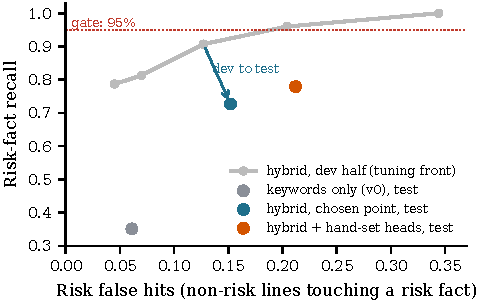
\includegraphics[width=\columnwidth]{fig_recall_front.pdf}
\caption{Risk recall against risk false hits. Grey: the tuning front on the dev half. Coloured: test-half results. The chosen point
loses 18 points of recall from dev to test.}
\label{fig:front}
\end{figure}

\textbf{Test results.} Table~\ref{tab:test}: hybrid matching doubled risk recall over tags at about two and a half times the false
risk hits, and hand-set heads added 5.2 points of recall for 6 more points of false hits. The 95\% target was missed. The ``none'' rate
did not move: every one of those false hits came from a tag (``tell me'', ``morning'' in ``Good morning'', ``today''), and
the embedding layer added no new false line.

\textbf{The tuning-to-test gap.} The chosen configuration scored 90.7\% risk recall at 12.7\% false hits on the dev half and 72.7\%
at 15.2\% on the test half (Fig.~\ref{fig:front}). An earlier configuration, tuned on dev after we had also added dev-inspired probes,
scored 98.7\% on dev and 72.7\% on test. The dev half was used twice (to write probes and to set five thresholds) on about 75 risk
pairs, which is enough to overfit.

\textbf{Recall-only tuning is unsafe.} An automatic re-tune that maximised dev risk recall chose a risk threshold that matched 34\% of
non-risk dev lines. In held-out conversations the patient model then treated ``How have you been sleeping, and how is your appetite?''
as a suicide question (the ``wouldn't wake up'' probes are close to sleep questions), answered about sleep but not appetite, and in
three of 98 turns volunteered the death wish unasked. Separating recall from strong matches and capping false risk hits fixed it.

\textbf{Trained alternatives that did not beat the rules.} (a) Linear heads on the frozen encoder, trained on 3,670 lines labelled by a
judge model (3,301 written by simulated clinician, student and provocateur doctors, 369 from session logs): the judge agreed with the
generator's intended topic on only 50.1\% of lines, and the heads reached a manner micro-F1 of 0.32 against 0.20 for keyword rules
but a topic micro-F1 of 0.66 against 0.69 for the language-model tagger on 381 judge-labelled held-out lines. A patient version using
them scored lower held-out. (b) A risk-topic detector trained on the generator's intended topics alone reached 0.87 recall but 0.35
precision for ``any risk'' in five-fold cross-validation. Noisy labels, not model capacity, were the limit.

\section{Discussion}
For a safety-relevant matcher, three practices mattered more than the encoder: a blind test set written without the tags; reporting
false risk hits next to risk recall; and a separate strict tier for actions with consequences (forcing a disclosure). Hand-set heads are
attractive when labels are scarce or noisy: they cost minutes, are fully inspectable, and keep fact text out of any weights, but here
they bought little. The next step is a small hand-checked label set and a fine-tuned encoder; the code for it exists but was not run.

\textbf{Limitations.} One writer produced the benchmark, and its labels are narrow; about 75 risk pairs per half make each recall figure
uncertain by several points; four cases in one language variety; the judge-labelled gold set was not hand-checked; latency was measured
on one laptop. Session logs used for training were the developer's own play-tests; the pipeline now admits only consented logs.

\section{Conclusion}
Hybrid matching with trust locks after matching doubles paraphrase recall of risk questions on a blind test set at modest cost, but
falls well short of what a safety gate needs, and a tuning half reused for probe writing overstates it by nearly twenty points.

\bibliographystyle{IEEEtran}
\bibliography{../shared/refs}

\end{document}
